\scanpage{46}

\[
\text{(vi)}\quad A_{\chi}(X\mathrm{x}Y)^0+A_{\chi}(Y\mathrm{x}Z)^0+\mathinner{\ldotp\ldotp\ldotp\ldotp}\ ,\quad\text{avec les mêmes notations .}
\]

Of course, the products and hyperplane sections are endowed with the polarizations stemming from the polarization on $X$. The conditions (v) and (vi) have tthe slight interest that they allow to express the conjecture $A(k)=C(k)$ in terms of $A(T)^0$ for every $T$ of even (resp. odd dimension), where the upper $0$ means that it is sufficient to look at what happens in critical dimensions.

For thenproof of the proposition, I told you already the equivalence of (i) and (ii),(ii bis). The equivalence of (iv) and (iv bis) is trivial by transposition, they \deleted{are of course implied by (i) because of the stabilities because $C_{\chi}(X)$ \unsure{et} $C_{\chi}(Y)$} imply (i) because $H^{2n-i}(X)\to H^i(X)$ is the compositum
\[
H^{2n-i}(X)\mathbin{-}H^{2n-i-2}(Y)\mathbin{-}H^i(Y)\mathbin{-}H^i(X
\]
where the extreme arrows are the ones of (iv bis) and (iv) and the middle one is induced by $\Lambda_Y^{(n-1)-i}$, and they are implied by (iii bis) because of the formula
\[
\deleted{\unsure{\varphi_*\varphi}}\quad(\Lambda_X\varphi_*)L_Y+L_X(\Lambda_X\varphi_*)=(\varphi_*\Lambda_Y\varphi^*+\operatorname{id}_X)\varphi_*\ .
\]
On the other hand $(\mathrm{iii})\Rightarrow(\mathrm{iii\ bis})$ is trivial, and so is $(\mathrm{i})\Longrightarrow(\mathrm{iii})$ because of the stabilities.
\margin{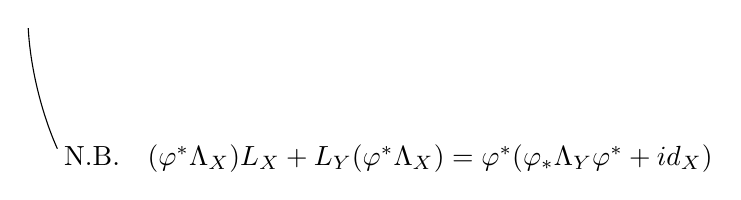
\begin{tikzpicture}[baseline=(nb.base)]\node[anchor=west,inner sep=0pt] (nb) at (0,0) {N.B.\quad $(\varphi^*\Lambda_X)L_X+L_Y(\varphi^*\Lambda_X)=\varphi^*(\varphi_*\Lambda_Y\varphi^*+\operatorname{id}_X)$};\draw (-.45,1.65) .. controls (-.42,1.10) and (-.26,.52) .. (-.08,.12);\end{tikzpicture}}

For the list of the known facts, you can state that :

1) In arbitrary caracteristics, $C(X)$ is known if $\dim X\leq2$, because more generally, it is known that in arbitray dimension $n$, $H^{2n-1}(X)\to H^1(X)$ is induced by an algebraic correspondance class; also, in arbitray dimension, it is known that $\pi_0,\pi_{2n},\pi_1,\pi_{2n-1}$ are algebraic (trivial for the first two, not quite trivial for the two next one's). If $\dim X=3$, it is not known however, even in \unsure{dim|car} $0$, if $C(X)$ or only $D(X)$ hold, nor $A(X)$ and $B(X)$ in car. $p>0$;
\inserted{also if for $1$-cycles, $\tau$-equiv. $=$ num. équivalence $\mathinner{\ldotp\ldotp\ldotp\ldotp}$}

\mspage{45}
